\chapter{State Consistency}
\label{chp:CONSISTENCY}

In order to design a state management and persistency architecture for P2P MMVEs, the requirements of such an architecture should first be understood. State management and persistency form part of the state consistency architecture of an MMVE. The requirements of the state management and persistency architecture, therefore, depends on what the state consistency architecture requires of it.

The role of this chapter is to describe the state consistency architecture in which the state management and persistency architecture will exist. The chapter provides a broad overview of consistency architecgure and also introduces a novel generic state consistency model that may be applied to both C/S and P2P network architectures to achieve state consistency in an MMVE. Classic state consistency architectures are also presented along with a discussion of how they fit into the generic architecture and their various advantages and disadvantages. Finally, the chapter presents an overview of the prevalant consistency model for P2P MMVE and discusses implementations of the various sections as they relate to the generic consistency model.

\section{The virtual environment}

A virtual environment can be characterised by its state, which consists of mutable or immutable objects. Immutable objects are those that cannot be altered, for example: rocks, hulls and trees. Mutable objects are those that can be altered, for example: NPCs, chests and doors. The \emph{environment state} (\emph{game state} when the environment is an online game) includes all positions, health and other attributes of all avatars, NPCs and other objects in the VE. Mutable objects may further be divided into ephemeral and permanent objects. Ephemeral objects need only be available for certain times, such as a player's (user agent's) avatar, when that avatar is online. Permanent objects should remain in the virtual world, whether the player who owns it is on-line or off-line, such as a house.

User agents are users (players) that connect to a VE. and non-user agents are AI scripts that implement NPC functionality. It is assumed that a single user agent is tied to a specific node in the network. Non-user agents can be hosted on any node and the hosting is an implementation of distributed computation, discussed in Section \ref{distributed_computation_requirement}. Both AI scripts and physical users may interact with the virtual world. When no distinction is required, the generic term ``agent'' is used.

When discussing how to segment VE state, it is sometimes easier to speak in terms of \emph{objects}, since they are separable. For the purposes of this work, objects are entities with both state and logic, which means they consume both storage space, as well as computing resources. Objects can also produce events, which should be sent to other objects. When this definition is used, NPC objects may be classified as a specific type of object, which forms part of the global environment state.

On a physical level, each computer that executes a virtual environment (VE) is executing a copy of the virtual environment. This is because a computer can only operate on what is stored in its primary memory. Because computers cannot access each other's primary memory banks, the necessity of multiple object copies is created. The existence of multiple object copies necessitates an object consistency model. In MMVEs, each computer uses the information of the virtual environment, stored in memory, to display the virtual environment to the user. The user makes decisions based on what is displayed and the executed operations on the environment. These operations can effect change in the environment and this change has to be communicated to all other entities capable of interacting with the environment. The fact that users operate on a local version of the environment and that the environment should appear the same to all users requires state consistency mechanisms.

\section{Event-logic-update cycle}
\label{event_logic_update}

It is impossible for multiple object states to always be consistent, because of the finite time taken to disseminate an object update that has occurred. A well designed object consistency model should no allow conflicting changes to local copies of object states.

An example of conflicting change is one actor in a virtual game world dealing five damage to another actor with five health. When the damage is dealt, the target actor is killed. If, however, the actor drank a potion that gives it some health, the damage dealt by the first player would not kill him. The state of the player being dead and the player being alive is not possible at the same time.

To overcome the difficulty of conflicting states, it was found that nodes participating in a VE should not be able to update the environment state directly. Nodes should rather express the effect they would like to have on the virtual world in terms of actions (events) and all nodes actions should then be combined by a third, centralised party, which then updates the state of the VE according to the combined causal actions of all nodes in the VE, to ensure that conflicts cannot occur. A disconnect is, thereby, created between the actions that can be performed on objects and the effect that the actions can have on objects. This is called the event-logic-update cycle \cite{}.

\emph{Events} are generated by objects and can be thought of as actions taken by agents, where agents can be humans or artificial intelligence (AI) scripts. These include casting a spell, using an item or walking.

\emph{Environment logic} is applied to events to determine what updates should be applied to the environment state. Environment logic is thus a ``think'' function, which determines how the environment should change as a result of an event. Another way to think about environment logic is to see it as the game rules.

An agent casting a spell might cause another agent's health to be reduced, her own health to be increased or a monster to spawn. When an agent is walking, the logic will cause the agent's position to update at the agent's walking speed.

Environment logic communicates how the world should change via \emph{state updates}. State updates are the incremental changes that specify how the environment state should change.

An object exists in two forms: the authoritative object and the non-authoritative object. The state of the authoritative object is considered to be the true state or absolute state. Copies of the authoritative object can be made, but these copies are all non-authoritative objects. If a discrepancy occurs between an authoritative object and a non-authoritative object, the state of the authoritative object is considered to be the true state. The work of the consistency mechanism in the VE is to ensure that all non-authoritative object states follows the authoritative object state within a time frame that is reasonable for the particular VE and the particular type of object.

Authoritative objects are the objects traditionally housed on the server in the C/S based MMVEs. All clients obtain replicas of these objects (termed the non-authoritative versions) and duplicate them locally in order to perform low latency computations. An example would be an NPC monster. When agents perceive the monster in the virtual world, a duplicate of the NPC objects is sent to the agent's computer for display purposes. When another agent attacks the NPC, the change in health will be computed at the server and an update is then sent in order to ensure consistency between authoritative and non-authoritative objects.

In P2P MMVEs there still exists a need for an authoritative object, but no centralised location exists to store that object. For each authoritative object, a peer is selected to store that object. That peer is termed the authoritative peer for the specific authoritative object it houses.

It should be noted that in this work, a node refers to a computer that is connected to a network, where a peer refers to a computer that is connected to a P2P network. Practically, there is no difference between a computer connected to a C/S network and one connected to a P2P network, except for the software that it executes.

\subsection{General flow}
\label{general_flow}

\begin{figure}[htbp]
 \centering
 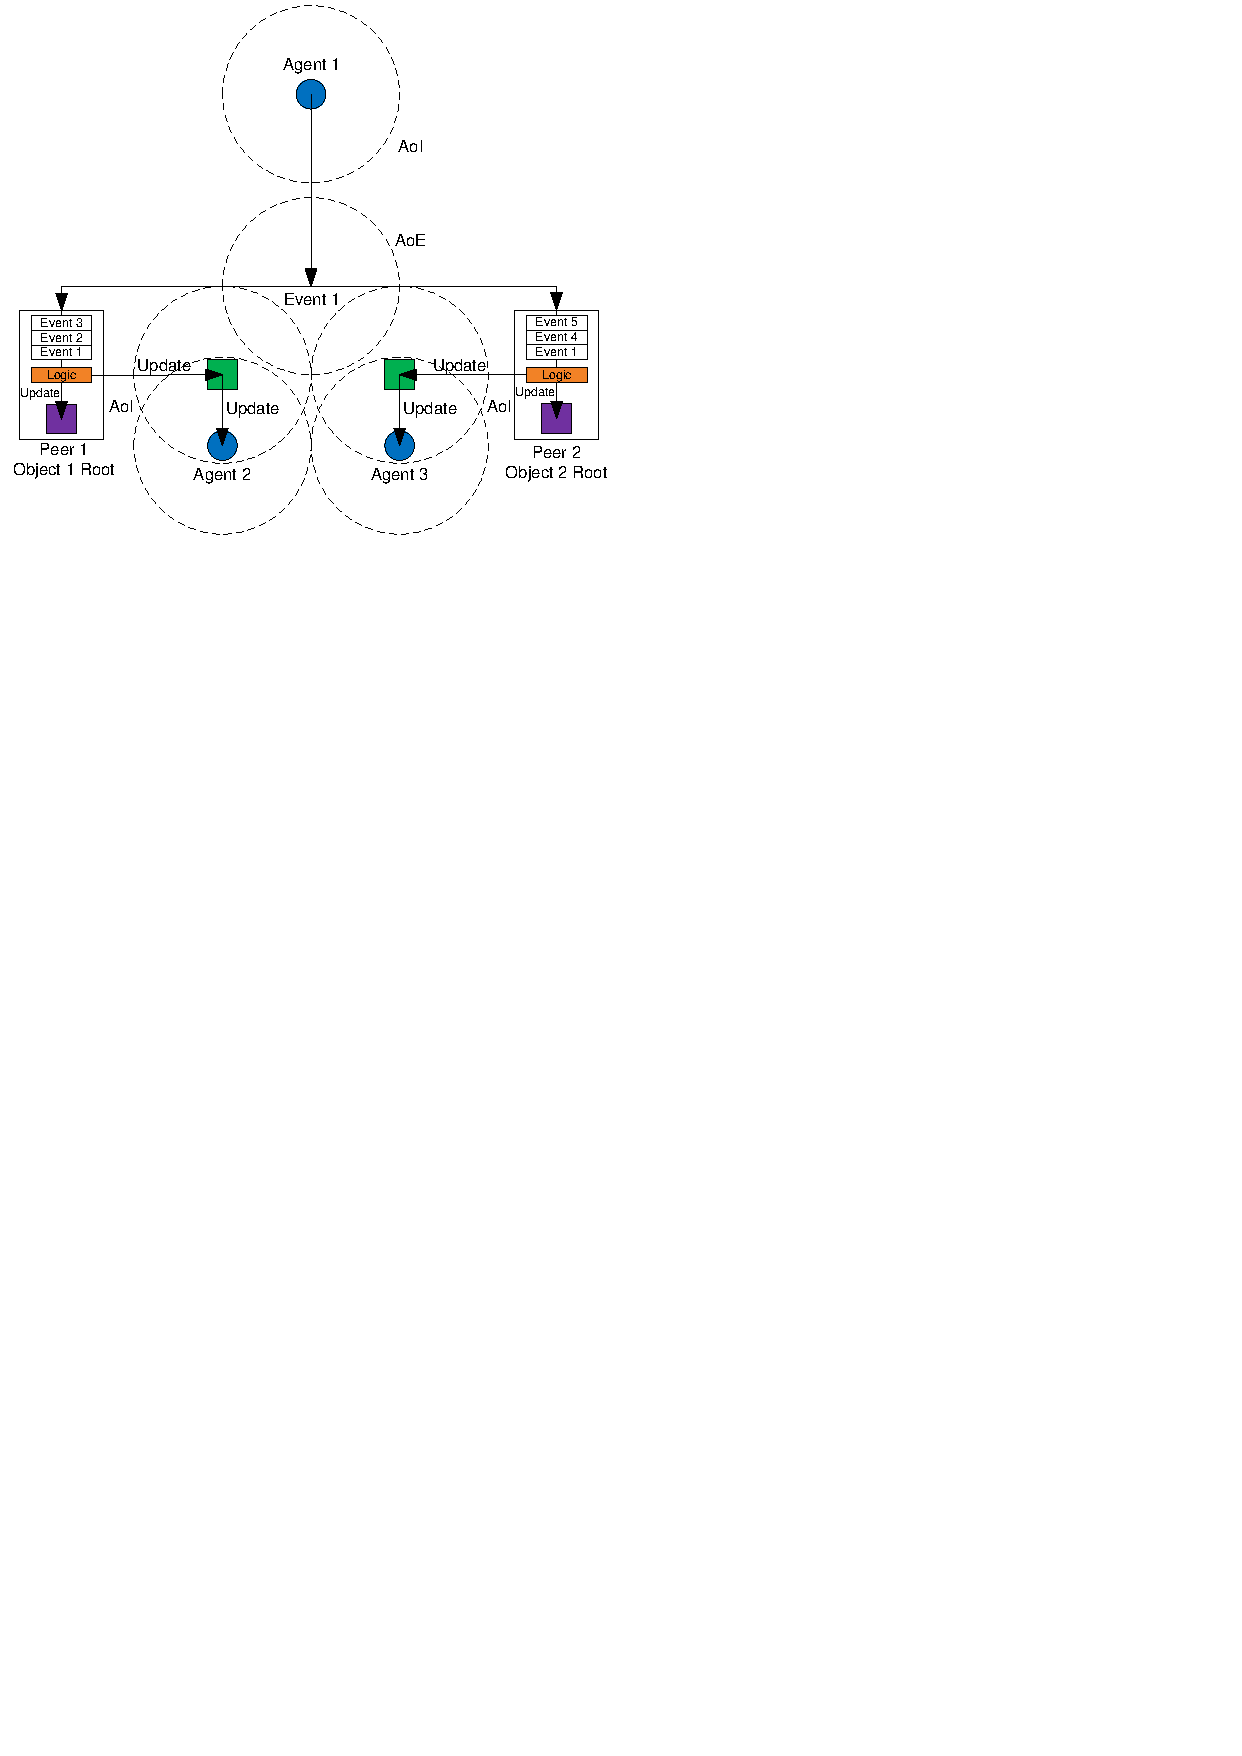
\includegraphics[clip=true, viewport=18mm 227mm 69mmm 292mm, width=0.6\textwidth]{generic_consistency_graphic}
 \caption{Graphic showing the flow of events and updates to achieve state consistency}
 \label{fig_event_update_flow_graphic}
\end{figure}

Figure \ref{fig_event_update_flow_graphic} depicts the flow of events and updates in response to the generation of an event by some agent. Agents are defined to be some form of intelligence that can interact with the virtual environment.

In Figure \ref{fig_event_update_flow_graphic}, Agent 1 generates Event 1 at the remote location shown. To maintain generality, events are defined to possess areas of effect (AoEs). An event's AoE determines which objects are in range to be potentially affected by an event. When an event's AoE encloses an object, that object is in range to be affected by the event. Whether the object is affected by the event, will be determined by the environment logic.

In Figure \ref{fig_event_update_flow_graphic}, Event 1 affect Object 1. Event 1 is, therefore, sent to Object 1's authoritative node, i.e. the node containing the authoritative copy of Object 1. Determining which objects are affected by an event is termed \emph{event layer interest management}. Delivering the event to the authoritative nodes of the affected object is termed \emph{event dissemination}. It should be noted that designs exist that use multiple authoritative objects, for example the event-based consistency model described in Section \ref{classic_event_based}, but that more research focus has been placed on consistency architectures where every object only possesses a single authoritative object, such as the update-based consistency model described in Section \ref{classic_update_based}.

When Event 1 arrives at Node 1, containing Object 1, the event is placed in a event queue in an order based on the time each event occurred. The process of determining which order events have to be processed in is called \emph{event ordering}, since many events will be arriving at an object's authoritative node from multiple agents simultaneously.

After event ordering has been performed, environment logic is applied to determine how a specific event will affect a specific object. To determine possible updates, that state of other objects might also have to be taken into account. An example is firing at an agent through a wall. If the thickness of the wall determines how much damage is delivered to the agent, the authoritative node processing the damage to the agent object will have to know the thickness of the wall.

When an event has been translated into a state update, the authoritative object on the authoritative node is updated. The new state of the object should also be communicated with all agents that can perceive the object in the virtual world. An object is perceived by an agent if the agent's area of interest (AoI)  in the VE encompasses the object. Every agent that can perceive an object, requires a non-authoritative copy of that object Determining which agents should receive object state updates is termed \emph{update layer interest management}. In the figure, Object 1 is perceived by Agent 2. Node 1 therefore has to send an update to the node containing agent 2. Delivering state updates to the affected agent nodes is termed \emph{update dissemination}.

When the update is delivered to Agent 2, the local object state is updated and the object's new state is displayed to the agent to allow the agent to make decisions and, therefore, generate events based on the new object state.

\subsection{Generic event-update model}
\label{generic_event_update_model}

To our knowledge, no papers exist that present a comprehensive picture of a state consistency architecture. In this chapter, papers will be discussed that individually implement all modules of the consistency architecture, but none were found to provide an overview of a state consistency model.

Since an overarching framework for state consistency was lacking in the literature, we developed the generic state consistency architecture, shown in Figure \ref{fig_event_update_flowdiagram}. This architecture allows us to put the literature regarding state consistency into context and allows us to identify requirements of the authoritative object store from a consistency perspective.

\begin{figure}[htbp]
 \centering
 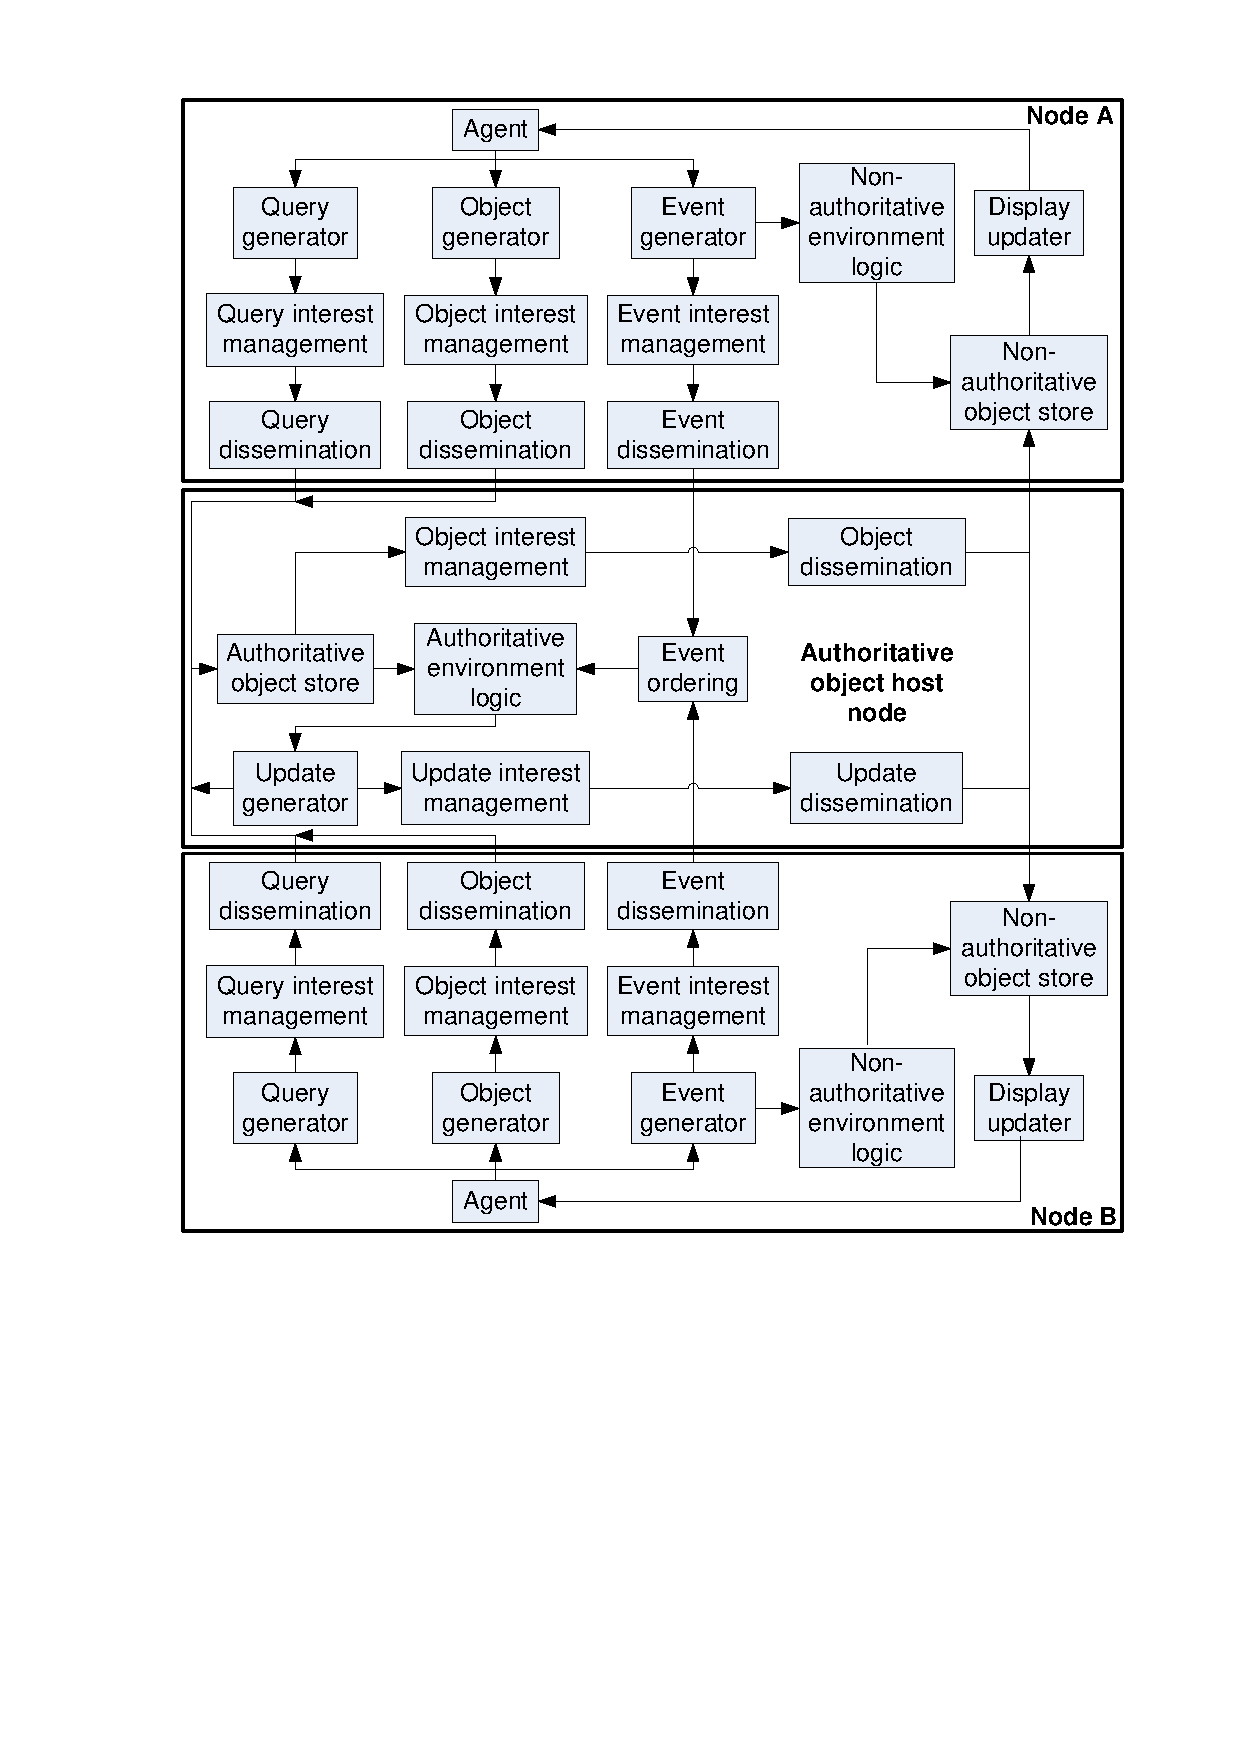
\includegraphics[clip=true, viewport=46mm 84mm 196mm 287mm, width=0.6\textwidth]{generic_consistency_flowdiagram}
 \caption{Flow diagram describing the event-update flow cycle and all steps required, from generating an event to delivering an update, to ensure object consistency.}
 \label{fig_event_update_flowdiagram}
\end{figure}

Figure \ref{fig_event_update_flowdiagram} shows the generic consistency flow diagram that ensures object state consistency.

\subsubsection{Agents and generators}

Agents generate three streams of requests, using a respective generator, that are sent to the authoritative object hosts: objects, events and queries.

Agents may be able to build structures, make clothes or construct a variety of mechanisms in the virtual world. The objects that the agent creates in this way should be stored on an authoritative peer.

Agents can also interact with the virtual environment and other agents, which are objects themselves. Agents interacting with objects generate events, which have to be sent to the authoritative peer.

Lastly, as agents more around in the virtual world, they might query an authoritative peer for any new objects that have entered their AoI. This is referred to as a range query and requires the retrieval of all objects within a certain area.

\subsubsection{Interest management and dissemination}

Interest management deals with finding a set of nodes that might have an interest in a request being generated. Events, objects and queries require some form of interest management.

Event interest management determines which objects will be affected by a generated event and on which authoritative nodes these objects are housed. Object interest management determines on which authoritative node the generated object should be stored. Query interest management has to discover which authoritative nodes contain objects that exist within the specified range.

Event, object and query dissemination deal with how information is sent to nodes after interest management determines which information should be sent (and to which nodes).

\subsubsection{Authoritative node}

All requests generated at non-authoritative nodes are sent to authoritative nodes for processing. Objects received are stored in the authoritative object store.

Multiple nodes, controlling different areas, may receive the same range query and be expected to supply the objects in their respective authoritative object stores that have positions that intersect with the range of the range query.

After receiving events, they are ordered to maintain causality. Object updates are generated from received events. An object update can be considered as some change that should be applied to a known object. Generating an object update, might also require the state of other objects, retrieved from the authoritative object store. Therefore, after the combination of event, object states and environment logic, an update is generated.

The authoritative node, therefore, can create two reply streams: objects and updates. Objects are created in response to queries and sent to the node requesting the objects. Updates are created in response to received events and these updates have to be applied to the object in the authoritative object store, as well to all non-authoritative copies of the updated object.

Update interest management determines which nodes require the generated update, which typically are the nodes whose agents can perceive the object in the virtual environment, and therefore posses non-authoritative copies of the object. Object interest management has to determine which node received a generated object. With a range query, this will merely be the node that sent the query, but other situation might occur where one node requests objects on behalf of another.

Update dissemination delivers a generated update to all nodes that contain local copies of the object. Multiple object updates may be generated for a single event. Any generated update may be delivered to multiple nodes that contain local copies of the object. Object dissemination delivers generated objects to the nodes that requested them.

\subsubsection{Discussion}

The flow diagram in Figure \ref{fig_event_update_flowdiagram} shows all steps that should be taken to ensure object consistency. We shall now demonstrate that the flow diagram of Figure \ref{fig_event_update_flowdiagram} is applicable to all known state consistency models of C/S as well as P2P MMVE architectures.

It should be noted that the generic consistency model is developed to fit all consistency architectures. To this end, some modules might be trivial in some consistency architectures, but become non-trivial with others. This is especially true for the C/S consistency model, where only a single server or server cluster exists, as will be described in Section \ref{classic_models}.

The differences between  the various architectures is where the authoritative objects are  housed, and how the authoritative peers are distributed. In a C/S system, all authoritative objects are housed in the server. In a P2P architecture, authoritative objects can be distributed on a number of peers, depending on the specific architecture. The various state consistency schemes for both C/S and P2P networks will be reviewed in the next sections.

\section{Classic consistency models}
\label{classic_models}

An overview of the two common models, currently used in MMVEs will be described. The models used in P2P MMVEs are all permutations of these two basic models. The two models are based on the two different network models. These are the fully distributed model, also called the event-based model \cite{p2p_cm_aoe}, and the C/S-based model, also called update-based model
\cite{unreal_networking}.

\subsection{Event-based (Fully distributed)}
\label{classic_event_based}

\begin{figure}[htbp]
\centering \subfloat[Event-based (fully distributed)]{\label{fig_p2p_cm}
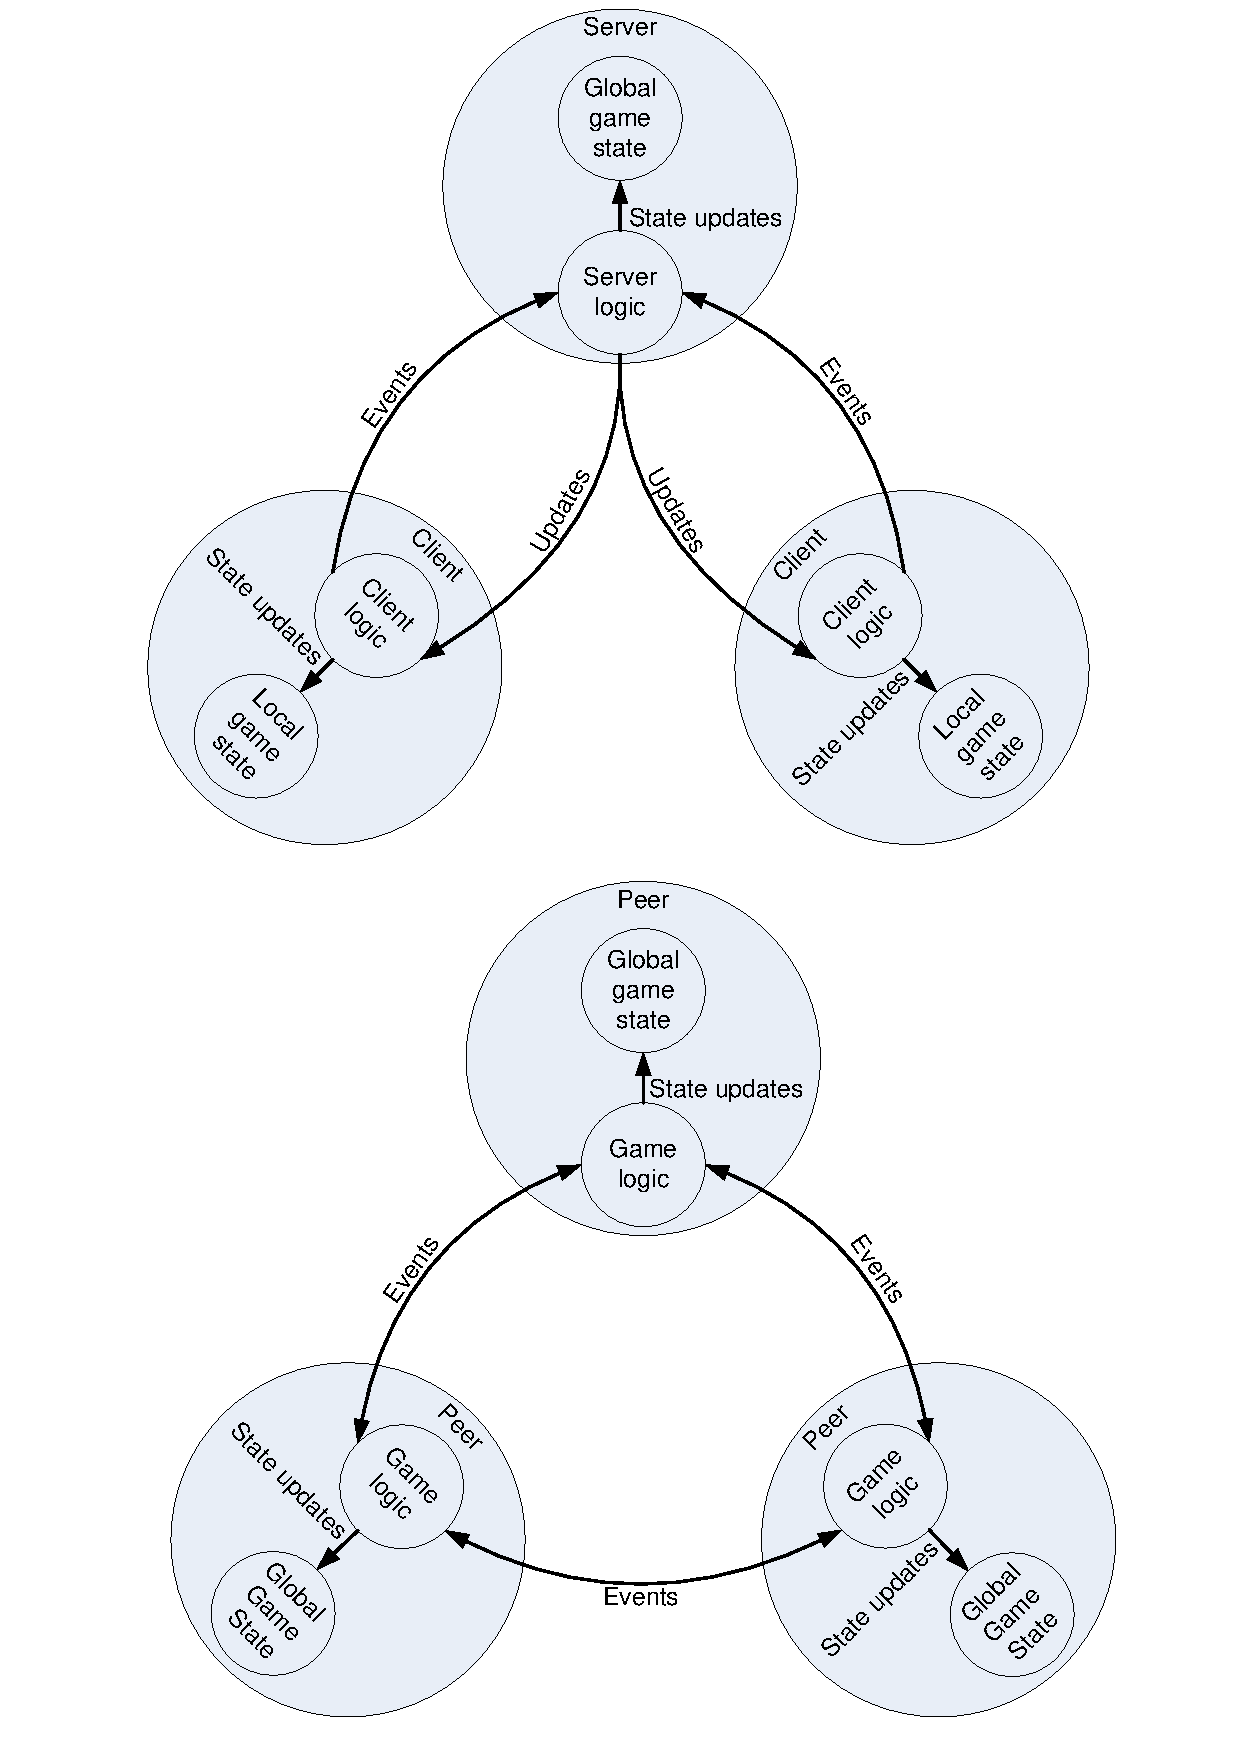
\includegraphics[clip=true, viewport= 2.5cm 0.5cm 19cm 15cm, width=0.5\columnwidth]{CS_P2P_CMs}}
 \subfloat[Update-based (client/server)]{\label{fig_cs_cm}
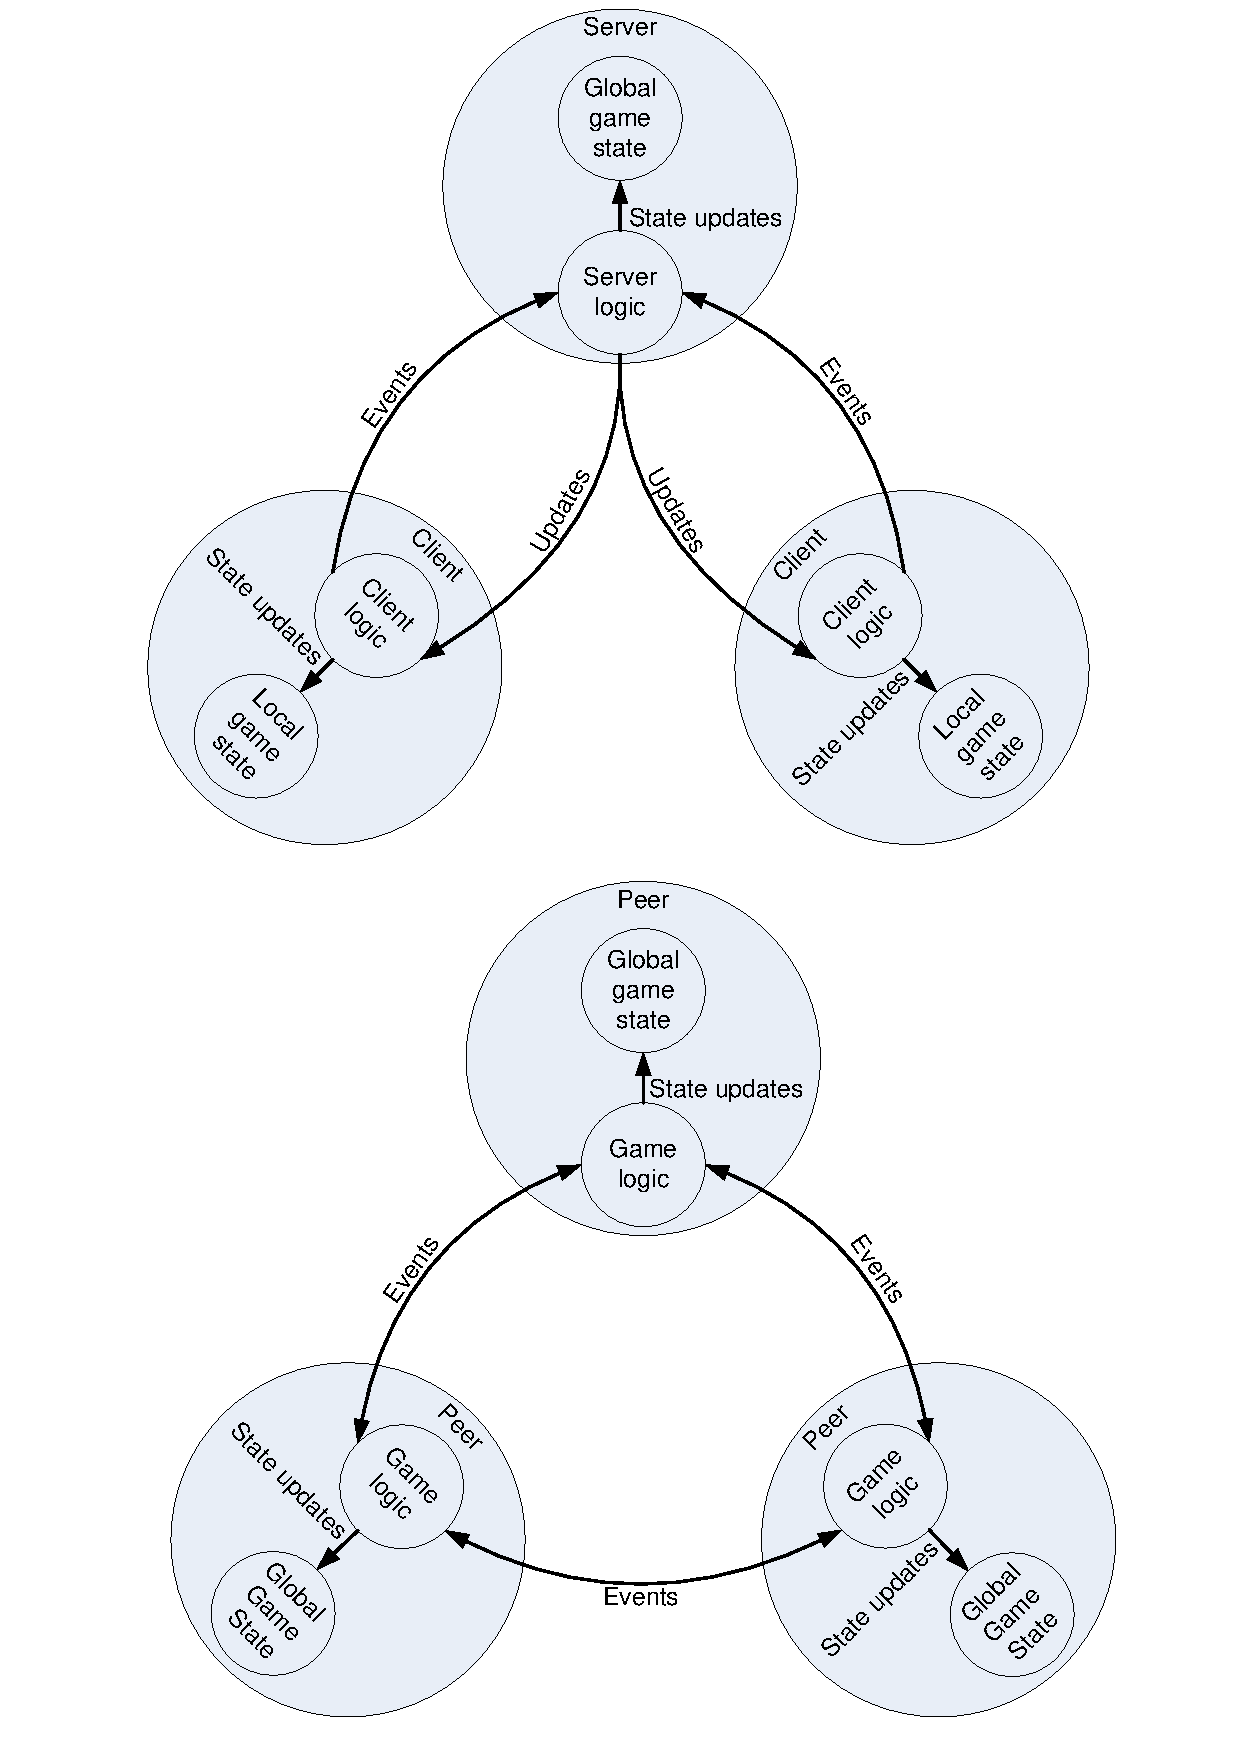
\includegraphics[clip=true, viewport= 2.5cm 15cm 19cm 30cm, width=0.5\columnwidth]{CS_P2P_CMs}}
\caption{Consistency models}
\end{figure}
%
Figure \ref{fig_p2p_cm} shows the fully distributed model. Each node has a copy of the global VE state. Any event that a node generates is sent to all other nodes. Each node processes all events separately and updates its own environment state accordingly. This consistency model is one where there exists multiple authoritative environment states.

The event-based model has fallen into disuse over the past few years, because of its lack of scalability and the slow down experienced when high latency nodes are connected. The slow down is necessary to maintain consistency.

\subsubsection{Event generation and dissemination}

With reference to the generic flow diagram in Figure \ref{fig_event_update_flowdiagram}, user agents access the VE using nodes in the fully connected network. Event generation occurs on nodes.

Event layer interest management is trivial, since all nodes receive all updates. Every node, therefore, requires an up-to-date list of all other nodes in the network. Event dissemination typically makes use of unicast to send all events to all nodes.

\subsubsection{Event ordering}
The order in which events are received is the same for all nodes, otherwise the environment states of different nodes may become inconsistent.
Usually some kind of lockstep technique is used to solve this issue \cite{pessimistic_lock_step}. The issue with lockstep is that it reduces the latency to twice that of the node with the highest latency.

Various techniques have been proposed that improves the latency by introducing some deadline before which all events should be submitted. An example of this is the New Event Ordering (NEO) technique \cite{cheat_proof_event_ordering}. Event ordering using deadlines makes it very difficult for a user with a high latency to access an MMVE, because if one user has a higher latency than the others and misses event deadlines, none of her actions will be processed by the other nodes which effectively excludes the user from the network.

An alternative to NEO is a P2P and C/S hybrid scheme, called the referee anti cheat scheme (RACS) \cite{cheating_taxonomy}. The scheme proposes referees, that are similar to the C/S network model, which allow for greater resistance to more types of cheats.

\subsubsection{Environment logic}
Complete environment logic is housed on every node, since every node must be able to apply the logic to translate any event into a state update. The environment logic will determine a set of objects that will be affected by the received event and update the affected objects accordingly.

\subsubsection{Update generation and dissemination}

The environment logic housed on every node generates state updates. These state updates are only used to update the local copies of affected objects, since each node is responsible for keeping its environment state up-to-date.

Update layer interest management and update dissemination is not required, since all affected nodes will have received the event.

\subsubsection{Authoritative object store}

The complete environment state is stored on each node.

\subsubsection{Advantages}
The event-based model works well for strategy games, and was implemented in Age of Empires \cite{p2p_cm_aoe} and Starcraft \cite{starcraft_network_model}.

When latency issues are not present and all users possess reasonable latencies, the event-based model can provide for an high-degree of responsiveness, because no extra latency is added by a server and no extra hop required to send information to a server which then relays it to all clients.

\subsubsection{Disadvantages}
The event-based model is not scalable, since all nodes must connect to all other nodes and all events are transmitted to
everyone. This means that as $N$, the number of nodes in the network increases, the traffic increases with a factor of $N^2$. The security issues of
the P2P network model, on which this consistency model is based, are also present. Slowdown is also experienced by all user if one user's
latency is below par, since the lockstep mechanism has to wait for all events to be received for that round to conclude \cite{cheat_proof_event_ordering}.

\subsubsection{Partially connected event-based consistency}
An even-based model that is not fully distributed might be considered, although such a model holds many challenges. Interest management techniques might be used to determine which nodes require updates. A challenge arises when nodes that were not aware of each other come into contact in the virtual world. A merge operation will have to be performed on the two authoritative environment states to ensure consistency. Such a model has not been proposed in practice and significant research will have to be performed into defining a framework that establishes relationships between events to maintain consistency. Such a system might be developed by defining classes of events and their interactions. A linear temporal logic model might then be developed to ensure consistent merging of states.

A partially connected model is not a classic consistency model.

\subsection{Update-based (C/S)}
\label{classic_update_based}

An alternative to the event-based model is the update-based model, shown in Figure \ref{fig_cs_cm}. This model is based on the C/S network model and based on the principle that only the server contains authoritative environment state.

\subsubsection{Event generation and dissemination}
Agents control clients that are able to generate events. As with classic event-based consistency, event layer interest management is trivial, since all events are sent to the server, usually making use of a unicast event dissemination technique. Interest management only becomes non-trivial when the P2P MMVE consistency model is considered in Section \ref{p2p_mmve_state_consistency}. The reasons why these sections exist in a discussion of the classic consistency models is to show that, although trivial, all sections relate to the generic consistency model.

\subsubsection{Event ordering}
\label{cs_event_ordering}

Event ordering is performed server-side, although it is not as critical as for the fully distributed model. If events are processed in different orders by different clients in the fully distributed model, the environment states of the clients will start to diverge and no mechanism currently exists to merge the diverging states.

If event ordering is not performed in the update-based model, the server might execute some events out of the order in which they were generated. The environment state will, however, remain consistent, since the server informs all clients of the environment state once it calculates a new environment state.

\subsubsection{Environment logic}
The environment logic that deals with high risk and high importance events is housed on the server. This allows for simplicity of design and increases system security, since the server can verify any actions performed by a client. Environment logic housed on the clients deal with low risk events that don't require a high level on consistency, for example, movement updates.

\subsubsection{Update generation and dissemination}

The environment logic generates states updates, which is used to update the server's authoritative environment state and is also used to inform nodes able to perceive the updated objects of the object's new state.

Update level interest management is required to determine which clients can perceive the updated objects. Unicast (direct transmission using TCP or UDP) is then used as update dissemination technique to inform the affected clients of the updated object states.

\subsubsection{Authoritative object store}
An authoritative global environment state is housed on the server and a  non-authoritative local environment state is housed on all clients for display purposes.

\subsubsection{Advantages}

\begin{itemize}
\item \emph{Authority}:The server state is authoritative, because if there is a conflict, the server state is always the state to which the system is expected to return. Combining server authority with the fact that the MMVE operator has full control over the server allows the operator to control who may access the server and on what terms.

\item \emph{Security}: The update-based model is secure, since clients cannot influence the state of any other clients and every client's state depends on updates received from the server.

\item \emph{Hardware scalability:} Another reason why the update based model is successful is because it is currently more scalable then the fully distributed model. More hardware can be used to build a more powerful server, which can handle more clients. It should be noted that scaling using hardware is expensive, since large server farms are required to host the VE.
\end{itemize}

\subsubsection{Disadvantages}


All disadvantages of the C/S architecture, as discussed in Section \ref{classic_cs_disadvantages}, are relevant to the update-based model, since the model is based on the C/S network model.
%
\begin{itemize}
\item The main disadvantage is the high cost involved in obtaining and maintaining the computer clusters and server hardware, required to host the VE.

\item When the server fails, the complete VE is off-line. Approaches exist to host the VE on multiple servers, but in this case a ``zone crash'' may still occur where a server hosting a specific region goes off-line. Additional redundancy is possible if backup servers are used, but this further increases costs.

\item Sufficient hardware may be made available to support the VE environment, but the update-based system struggles with dynamic load balancing to cope with large numbers of users flocking to a single area in a short span of time \cite{flocking}.
\end{itemize}

\section{P2P MMVE state consistency models}
\label{p2p_mmve_state_consistency}

Various schemes have been proposed to address the various challenges of P2P MMVE state consistency, but these have mostly occurred in isolation, each approach focussing on a few of the requirements, but not addressing all requirements as identified in Section \ref{generic_event_update_model}. Some of the proposed schemes will be reviewed.

What should be noted is that the various areas of state consistency, e.g. interest management, event ordering, state management, and the other areas discussed in Section \ref{generic_event_update_model}, are quite modular, which might allow for the integration of the best schemes in each area into a comprehensive P2P MMVE state consistency model.

The most complete P2P MMVE state consistency model found was P2P Second Life.

P2P MMVE schemes are based on one of the two classic consistency models described in Section \ref{classic_models}. Although it might seem that the fully distributed model is a better fit for P2P MMVE state consistency, this model has received less attention than the C/S model. The reason for this is partly because of the difficulties in getting the fully distributed model to scale. Usually the fully distributed model makes use of rounds, where users submit events and all user events are executed at the end of a round. In an MMVE with tens of thousands to millions of users, designing the round mechanism to remain scalable is a challenge. Rounds are required, because of the event ordering mechanism that ensures state consistency.

The C/S consistency architecture is applied to P2P MMVEs by distributing authoritative objects. Every authoritative object is maintained by a single peer, that receives all events for the object, applies the environment logic and informs all peers of the generated updates. This effectively creates a C/S consistency model from the perspective of each authoritative object. An example of such a consistency model is the region-based model, described next.

In P2P networks, some peers may be selected as super peers. Super peers are specialised peers that perform specialised tasks within the P2P network. The super peer is selected in some logical way, from the available set of peers and then promoted. Super peer selection in itself is a complex topic that has to deal with determining whether a peer has sufficient resources available and also whether the peer is trustworthy.

A region is usually created by segmenting the world, with super peers acting as regional servers to all peers in their region. Each super peer receives all events, handles all environment logic and distributes updates to all peers in its region. The super peer also handles state management and persistency for its region, containing NPCs, objects and persistent user data. Clients in the region only house copies of the regional objects and some client logic to update the local copies of objects.

\begin{figure}[htbp]
 \centering
 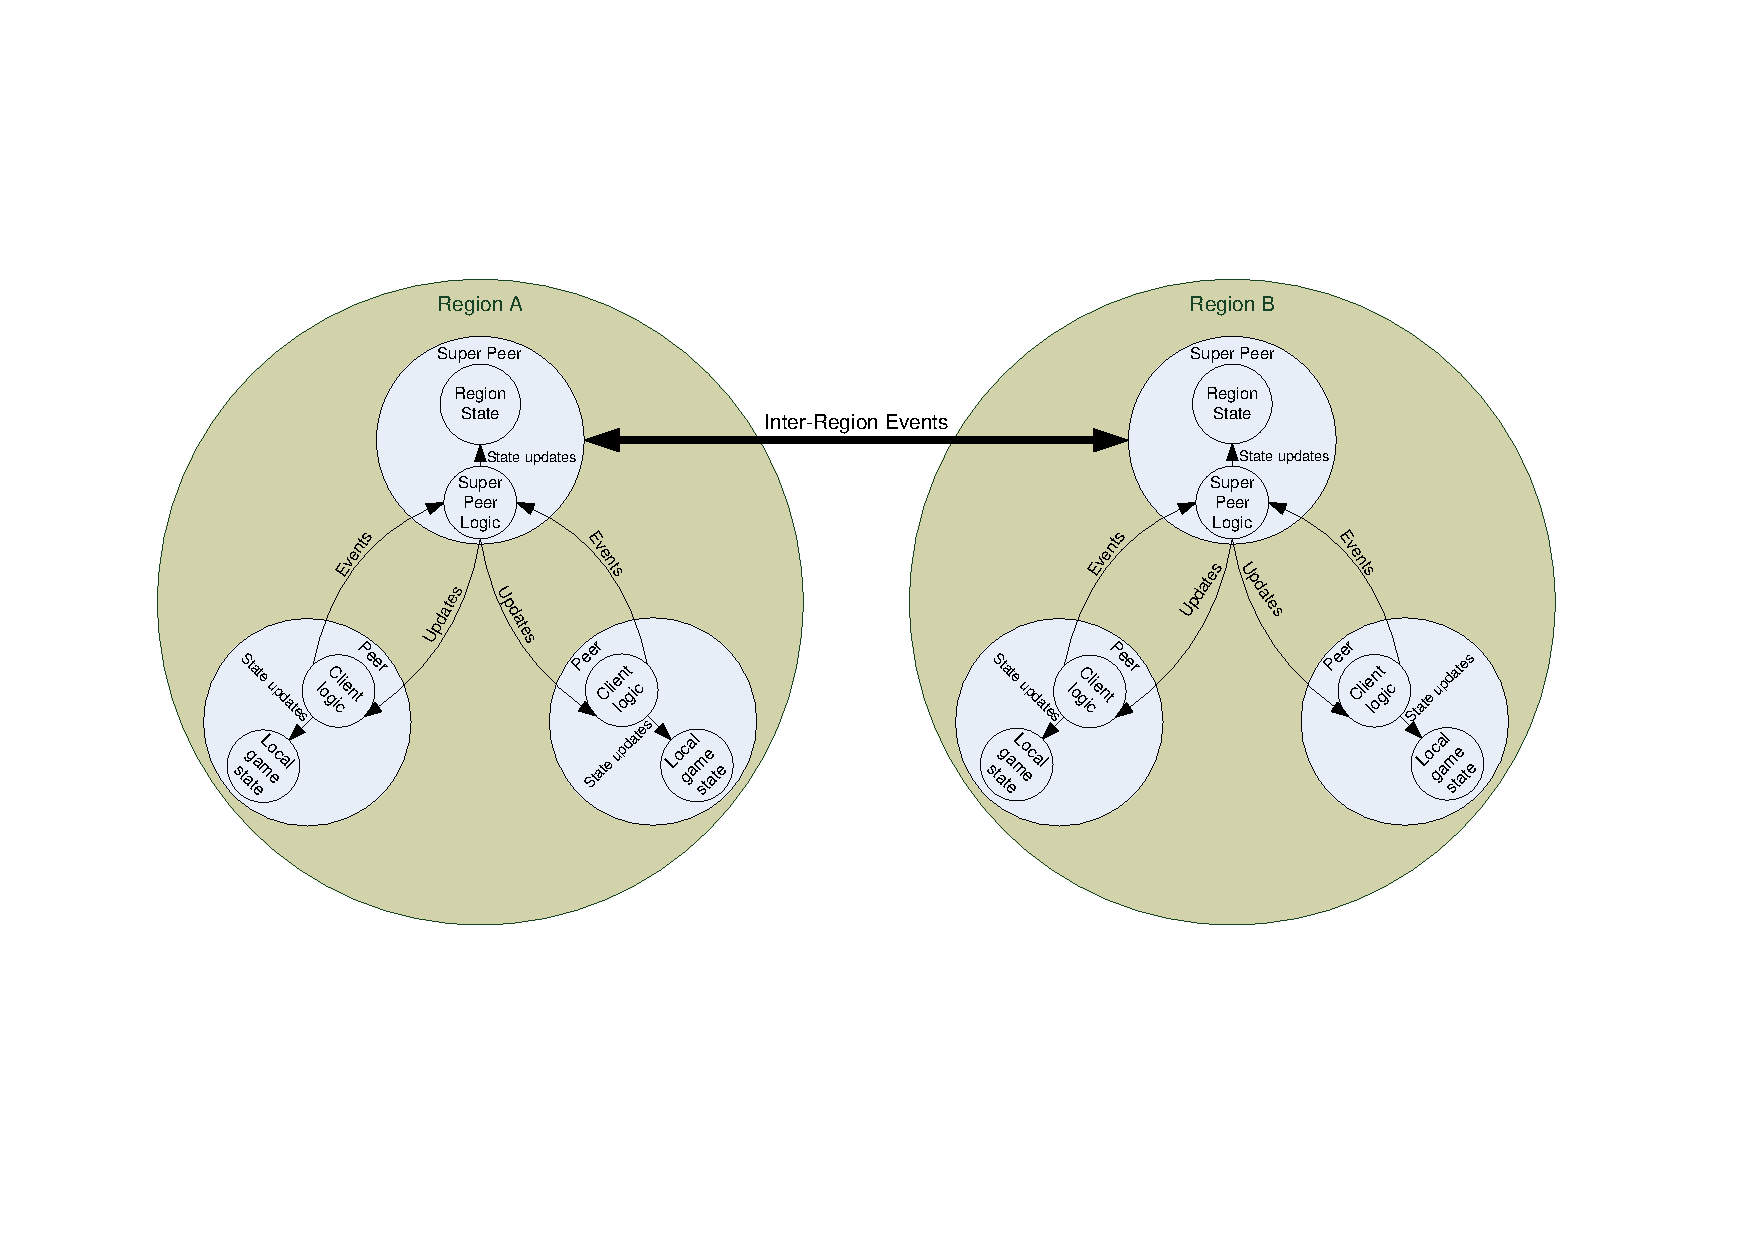
\includegraphics[clip=true, viewport=2cm 5cm 27cm 16.5cm, width=\textwidth]{region_based_CS_CM}
 \caption{Region-based Client/Server consistency model}
 \label{fig_cs_region_cm}
\end{figure}
%
The consistency model is depicted in Figure \ref{fig_cs_region_cm}. One can see that this approach is modelled on the update based model, but segmented into separate regions. The role of the server is here fulfilled by a super peer.

Presented here is an overview of the different techniques and general trends present in the various areas of P2P MMVEs. The overview does not presume to present an exhaustive list of papers in these areas, rather to place the topic of state management and state persistency in context.

%Include the actual consistency models here. Region-based update-based, fully distributed

\subsection{Event generation and dissemination}

In P2P networks, each peer contains an agent that represents a user (player). Each peer can, therefore, generate events that have to be transmitted to the peers containing the authoritative objects affected by the generated event.

Classically, application level multicast (ALM) and unicast techniques are the two methods of event dissemination. The specific technique used depends on the grain of the event dissemination. ALM is used, instead of router level multicast, because of a lack of general support for this technology at the router level \cite{ip_multicast_deployment_issues}.

ALM is used for coarsely grained interest management techniques, while unicast is used for finely grained techniques. Unicast is not used for coarsely grained techniques, because it is not scalable. For a network containing $N$ peers, $N^2$ messages are exchanges for every user action. ALM, however, significantly increases the message latency in the system, because messages first have to be routed over a structured overlay network. ALM is however preferred over unicast for large numbers of messages, because of the weak scalability of unicast.

An ALM scheme has recently been proposed, that sends updates to locations in the virtual world, rather than to specific users \cite{Ghaffari_Delaunay_churn_mobility}. This removes the need to first determine which peers will be affected by an event, before the event may be transmitted. Another ALM scheme proposed sends messages to the neighbours in the AoI, instead of to all the users in the region \cite{Seeger_area_based_gossip_multicast}. This effectively implements a basic interest management scheme, where only neighbouring users can receive events.

\subsection{Event ordering}

The presence and complexity of event ordering depends on the consistency architecture on which the P2P MMVE is based. In systems that use the update-based (C/S) model, no papers have addressed the issue of event ordering, since events delivered out of order will not lead to an inconsistent state, as discussed in Section \ref{cs_event_ordering}.

Where distributed architectures are proposed for P2P MMVEs, event ordering is of high importance. Designers of P2P MMVEs make use of the same event ordering mechanisms, as is used in the fully distributed model \cite{hybrid_storage1}.

To support a large number of users using an event-based model, event ordering with the concept of interest has been developed using N-trees \cite{GauthierDickey_ntrees}.

\subsection{Environment logic}

In P2P architectures, the environment logic for all objects have to be housed on all peers, since any peer can be selected to store any object. The environment logic itself is, therefore, usually also distributed as part of the client software. This does not mean that the environment logic cannot change, but any change in environment logic will be in the form of a client patch, which occurs while the application is off-line.

\subsection{Update generation and dissemination}

In P2P MMVEs, update generation is the responsibility the peer containing the authoritative object. When the peer receives an event, environment logic is applied to generate an update. This update is then disseminated to all peers that have local non-authoritative copies of the object. This is similar to the update-based consistency model discussed in Section \ref{classic_update_based}.

\subsection{Update and event layer interest management}
\label{key_challenges_im}

Interest management occurs both in the update and the event layer. For the event layer, the set of peers housing the authoritative object, affected by the generated event, has to determined. For the update layer, the set of peers has to be found which house the agents that will perceive an object update. What is common to both layers is that a message has to be sent to a subset of peers with interest in the message and the interest management mechanism must determine what that subset is.

Thus far in P2P MMVE literature, little attention has been paid to whether the interest management in question is developed for the event layer or the update layer. Most discussions implicitly assume a layer and all the descriptions of the algorithm are based around the terminology of that layer. That is not to say that the algorithm itself might not be traversable to the other layer, just that this is not discussed.

Interest management is used to determine the smallest amount of information that a peer requires, in order to present an accurate representation of the world to users. In consistency terms, it provides a means to determine which non-authoritative objects require updates of the authoritative object. The idea is not specific to P2P MMVEs and was already formally suggested in \cite{First_IM} and later with greater focus on a distributed environment in \cite{Whang_agent_based_IM}.

The main idea is that a user has a limited visual range and area around the user in which it can interact with objects. The user requires update information of all objects in this area, called the user's Area of Interest (AoI). AoI calculations also rely on the fact the a user's direction and velocity of movement cannot change instantaneously and are bounded in magnitude.

Extensive research has been done into solving AoI problems and a comparison of techniques can be found in \cite{Boulanger_IM_compare} and \cite{IM_and_ED_survey_Krause}. The solutions range from aura/nimbus \cite{Benford_spatial_IM} to publish/subscribe  \cite{mercury_publish_subscribe} to Voronoi based models \cite{Hu_voronoi_IM},  \cite{Buyukkaya_voronoi_state_management} to hybrid models \cite{hybrid_IM}, \cite{MOPAR}, \cite{fan_mediator_paper}.

Generally, interest management solutions can be divided into coarsely or finely grained solutions, although the hybrid models, especially MOPAR, seem to have gained greater popularity because they seem to have all the benefits of the two solutions and little of the drawbacks \cite{MOPAR}. MOPAR has been shown to perform better than either a finely grained technique or a coarsely grained technique.

Coarsely grained solutions usually divide the virtual environment into multiple regions and when a user enters a region, it subscribes to that region's events. This is called the region-based publish subscribe model \cite{Fan_deisgn_issues_p2p}. All users in the region then receive the region's events, even for users not in their AoI.

Finely grained techniques create groups of agents based on their AoIs. Groups of interacting agents directly exchange information, so all agents only receive information that is relevant to them. This has been termed the spatial model \cite{Fan_deisgn_issues_p2p}. The grain of the solution in turn determines the type of event dissemination that should be used, as described later in this section.

Another example of finely grained interest management, making use of frontier sets, was presented in \cite{IM_frontier_sets} and implemented in Quake 3. By using Frontier Sets, it is possible to describe an area in which an agent may move, where no other users will require updates of that movement. Conversely, a set of other users that require movement updates from a specific user is also given by the frontier set.

MOPAR partitions the VE into hexagonal regions and appoints ``home'' peers to act as bootstrap peers for each region. A home peer of a region is that peer whose ID is the closest match the the region ID. This allows any peer to find the home peer for a region. A master peer is then selected for every region, whose function it is to inform slave peers of new neighbours. All slaves peers in a region register at their region's master peer.

Slave peers send direction and velocity updates to their masters. Masters communicate directly with other masters if a peer is about to enter their region. Masters inform their slaves of a new neighbour. Slaves communicate directly with each other, once identified by a master.

Interest management is a mature area of research, with many proposed schemes. It is one of the areas in P2P MMVE research that has received the most attention.

\subsection{Authoritative object store}

In a recently completed PhD on the subject of P2P MMVEs, Lu Fan had this to say about state persistency: ``Game state persistency is a major challenge for P2P MMVEs as existing P2P storage infrastructures are designed to support file sharing, and seldom fulfil the performance and security requirements of a MMVE. \ldots the persistency area is still immature with many problems waiting to be investigated.'' \cite{Fan_phd}.

State persistency is treated as a sub domain of state consistency and is similar to state management, as discussed in Section \ref{management_persistency_def}. State models define where and how the authoritative objects are stored. It is assumed that non-authoritative objects are always stored in the primary memory of the clients that immediately require the information contained in the authoritative object.

The most mature state management model reviewed is that of P2P Second Life.
%Describe P2P Second Life.

\section{Conclusion}

This chapter introduced the event-update consistency model that is mostly used in MMVE. From the literature reviewed, a generic process was developed that will ensure state consistency. Classic state consistency models were introduced and it was shown how these models relate to the generic state consistency process. After this, state consistency for P2P MMVEs were described. It was shown how the models used are all based on the classic consistency models. Some research into every area of P2P MMVE state consistency was discussed to enable the reader to place the work done here, into perspective.

In this chapter it was shown that the field of P2P MMVE state consistency is a growing one, already containing many significant contributions. But is was also shown that there is still much room for improvement on how we think about state management and state persistency and that there are still many open questions in these fields.
